\documentclass{standalone}
\usepackage{tikz}
\usetikzlibrary{patterns, positioning}

\begin{document}
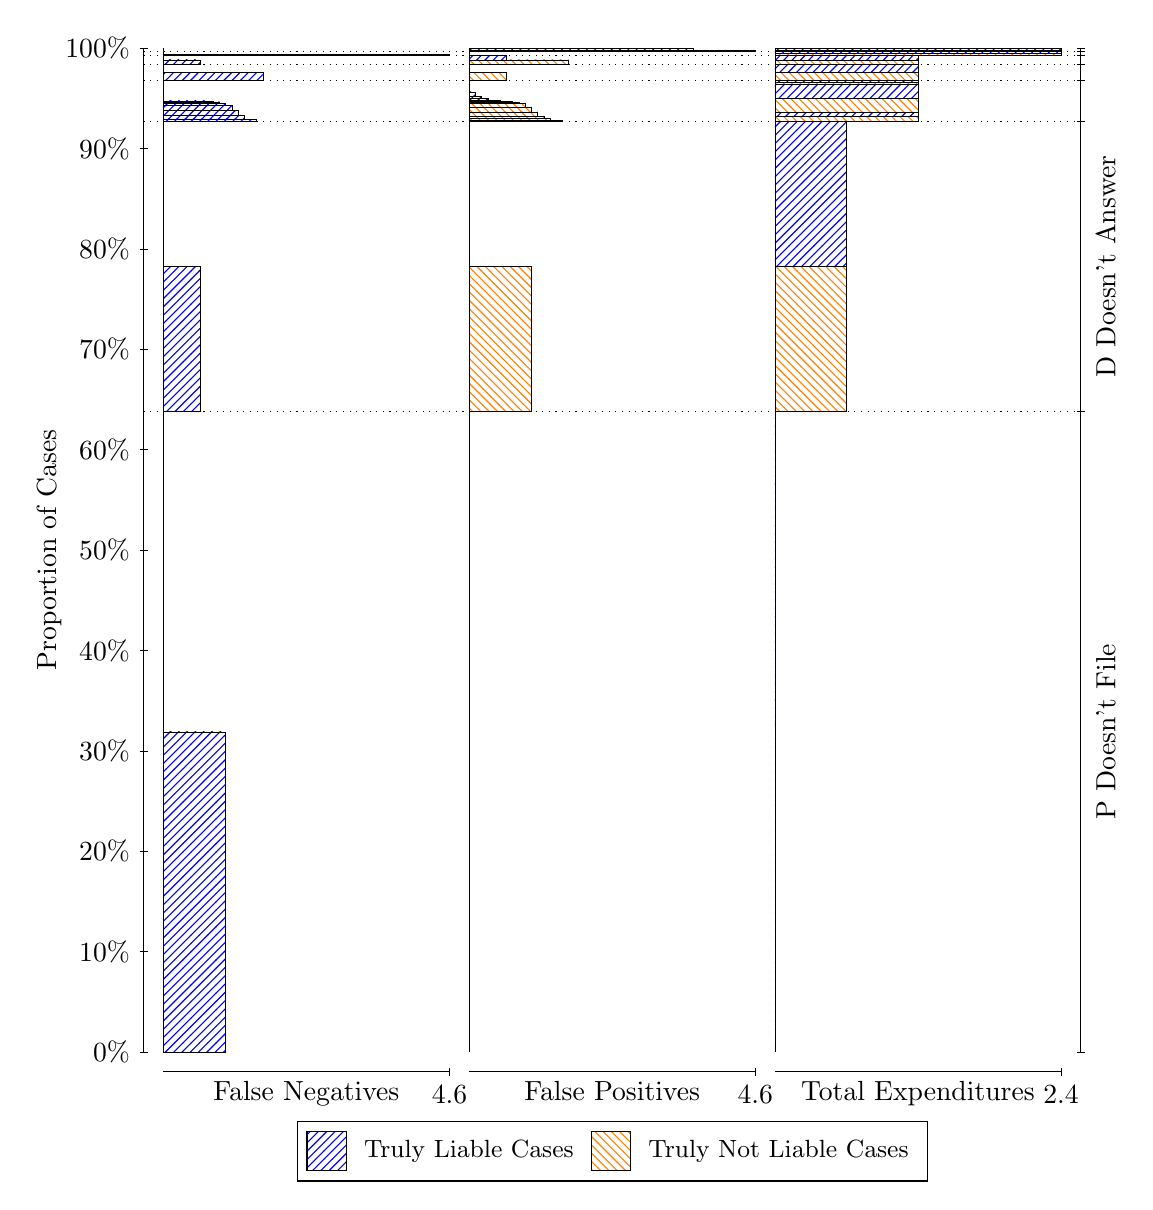
\begin{tikzpicture}
\draw[black, very thin] (1.5,1.75) -- (1.5,14.5);
\node[rotate=90, anchor=center] at (0.3, 8.125) {Proportion of Cases};
\draw[black, very thin] (1.45,1.75) -- (1.55,1.75);
\node[anchor=east] at (1.45, 1.75) {0\%};
\draw[black, very thin] (1.45,3.025) -- (1.55,3.025);
\node[anchor=east] at (1.45, 3.025) {10\%};
\draw[black, very thin] (1.45,4.3) -- (1.55,4.3);
\node[anchor=east] at (1.45, 4.3) {20\%};
\draw[black, very thin] (1.45,5.575) -- (1.55,5.575);
\node[anchor=east] at (1.45, 5.575) {30\%};
\draw[black, very thin] (1.45,6.85) -- (1.55,6.85);
\node[anchor=east] at (1.45, 6.85) {40\%};
\draw[black, very thin] (1.45,8.125) -- (1.55,8.125);
\node[anchor=east] at (1.45, 8.125) {50\%};
\draw[black, very thin] (1.45,9.4) -- (1.55,9.4);
\node[anchor=east] at (1.45, 9.4) {60\%};
\draw[black, very thin] (1.45,10.675) -- (1.55,10.675);
\node[anchor=east] at (1.45, 10.675) {70\%};
\draw[black, very thin] (1.45,11.95) -- (1.55,11.95);
\node[anchor=east] at (1.45, 11.95) {80\%};
\draw[black, very thin] (1.45,13.225) -- (1.55,13.225);
\node[anchor=east] at (1.45, 13.225) {90\%};
\draw[black, very thin] (1.45,14.5) -- (1.55,14.5);
\node[anchor=east] at (1.45, 14.5) {100\%};

\draw[black, very thin] (13.4,1.75) -- (13.4,14.5);
\draw[black, very thin] (13.35,1.75) -- (13.45,1.75);
\node[anchor=west] at (13.35, 1.75) {};
\draw[black, very thin] (13.35,9.8818) -- (13.45,9.8818);
\node[anchor=west] at (13.35, 9.8818) {};
\draw[black, very thin] (13.35,13.571) -- (13.45,13.571);
\node[anchor=west] at (13.35, 13.571) {};
\draw[black, very thin] (13.35,14.085) -- (13.45,14.085);
\node[anchor=west] at (13.35, 14.085) {};
\draw[black, very thin] (13.35,14.296) -- (13.45,14.296);
\node[anchor=west] at (13.35, 14.296) {};
\draw[black, very thin] (13.35,14.402) -- (13.45,14.402);
\node[anchor=west] at (13.35, 14.402) {};
\draw[black, very thin] (13.35,14.454) -- (13.45,14.454);
\node[anchor=west] at (13.35, 14.454) {};
\draw[black, very thin] (13.35,14.5) -- (13.45,14.5);
\node[anchor=west] at (13.35, 14.5) {};

\draw[black, very thin, pattern color=blue, pattern=north east lines] (1.75,1.75) rectangle (2.5399,5.8159);
\draw[black, very thin, pattern color=orange, pattern=north west lines] (1.75,5.8159) rectangle (1.75,9.8818);
\draw[black, very thin, pattern color=blue, pattern=north east lines] (1.75,9.8818) rectangle (2.2239,11.728);
\draw[black, very thin, pattern color=orange, pattern=north west lines] (1.75,11.728) rectangle (1.75,13.571);
\draw[black, very thin, pattern color=blue, pattern=north east lines] (1.75,13.571) rectangle (2.9348,13.589);
\draw[black, very thin, pattern color=blue, pattern=north east lines] (1.75,13.589) rectangle (2.8558,13.599);
\draw[black, very thin, pattern color=blue, pattern=north east lines] (1.75,13.599) rectangle (2.7768,13.648);
\draw[black, very thin, pattern color=blue, pattern=north east lines] (1.75,13.648) rectangle (2.6978,13.712);
\draw[black, very thin, pattern color=blue, pattern=north east lines] (1.75,13.712) rectangle (2.6188,13.77);
\draw[black, very thin, pattern color=blue, pattern=north east lines] (1.75,13.77) rectangle (2.5399,13.799);
\draw[black, very thin, pattern color=blue, pattern=north east lines] (1.75,13.799) rectangle (2.4609,13.816);
\draw[black, very thin, pattern color=blue, pattern=north east lines] (1.75,13.816) rectangle (2.3819,13.822);
\draw[black, very thin, pattern color=blue, pattern=north east lines] (1.75,13.822) rectangle (2.3029,13.829);
\draw[black, very thin, pattern color=orange, pattern=north west lines] (1.75,13.829) rectangle (1.75,14.085);
\draw[black, very thin, pattern color=blue, pattern=north east lines] (1.75,14.085) rectangle (3.0138,14.188);
\draw[black, very thin, pattern color=orange, pattern=north west lines] (1.75,14.188) rectangle (1.75,14.296);
\draw[black, very thin, pattern color=blue, pattern=north east lines] (1.75,14.296) rectangle (2.2239,14.35);
\draw[black, very thin, pattern color=orange, pattern=north west lines] (1.75,14.35) rectangle (1.75,14.402);
\draw[black, very thin, pattern color=blue, pattern=north east lines] (1.75,14.402) rectangle (5.3833,14.422);
\draw[black, very thin, pattern color=orange, pattern=north west lines] (1.75,14.422) rectangle (1.75,14.454);
\draw[black, very thin, pattern color=orange, pattern=north west lines] (1.75,14.454) rectangle (1.75,14.472);
\draw[black, very thin, pattern color=blue, pattern=north east lines] (1.75,14.472) rectangle (1.75,14.5);
\draw[black, very thin, pattern color=orange, pattern=north west lines] (5.6333,1.75) rectangle (5.6333,5.8159);
\draw[black, very thin, pattern color=blue, pattern=north east lines] (5.6333,5.8159) rectangle (5.6333,9.8818);
\draw[black, very thin, pattern color=orange, pattern=north west lines] (5.6333,9.8818) rectangle (6.4232,11.725);
\draw[black, very thin, pattern color=blue, pattern=north east lines] (5.6333,11.725) rectangle (5.6333,13.571);
\draw[black, very thin, pattern color=orange, pattern=north west lines] (5.6333,13.571) rectangle (6.8181,13.577);
\draw[black, very thin, pattern color=orange, pattern=north west lines] (5.6333,13.577) rectangle (6.7391,13.584);
\draw[black, very thin, pattern color=orange, pattern=north west lines] (5.6333,13.584) rectangle (6.6601,13.602);
\draw[black, very thin, pattern color=orange, pattern=north west lines] (5.6333,13.602) rectangle (6.5812,13.631);
\draw[black, very thin, pattern color=orange, pattern=north west lines] (5.6333,13.631) rectangle (6.5022,13.688);
\draw[black, very thin, pattern color=orange, pattern=north west lines] (5.6333,13.688) rectangle (6.4232,13.75);
\draw[black, very thin, pattern color=orange, pattern=north west lines] (5.6333,13.75) rectangle (6.3442,13.797);
\draw[black, very thin, pattern color=orange, pattern=north west lines] (5.6333,13.797) rectangle (6.2652,13.807);
\draw[black, very thin, pattern color=orange, pattern=north west lines] (5.6333,13.807) rectangle (6.1862,13.826);
\draw[black, very thin, pattern color=blue, pattern=north east lines] (5.6333,13.826) rectangle (6.0283,13.833);
\draw[black, very thin, pattern color=blue, pattern=north east lines] (5.6333,13.833) rectangle (5.9493,13.84);
\draw[black, very thin, pattern color=blue, pattern=north east lines] (5.6333,13.84) rectangle (5.8703,13.857);
\draw[black, very thin, pattern color=blue, pattern=north east lines] (5.6333,13.857) rectangle (5.7913,13.886);
\draw[black, very thin, pattern color=blue, pattern=north east lines] (5.6333,13.886) rectangle (5.7123,13.943);
\draw[black, very thin, pattern color=blue, pattern=north east lines] (5.6333,13.943) rectangle (5.6333,14.085);
\draw[black, very thin, pattern color=orange, pattern=north west lines] (5.6333,14.085) rectangle (6.1072,14.193);
\draw[black, very thin, pattern color=blue, pattern=north east lines] (5.6333,14.193) rectangle (5.6333,14.296);
\draw[black, very thin, pattern color=orange, pattern=north west lines] (5.6333,14.296) rectangle (6.8971,14.348);
\draw[black, very thin, pattern color=blue, pattern=north east lines] (5.6333,14.348) rectangle (6.1072,14.402);
\draw[black, very thin, pattern color=orange, pattern=north west lines] (5.6333,14.402) rectangle (5.6333,14.434);
\draw[black, very thin, pattern color=blue, pattern=north east lines] (5.6333,14.434) rectangle (5.6333,14.454);
\draw[black, very thin, pattern color=orange, pattern=north west lines] (5.6333,14.454) rectangle (9.2667,14.472);
\draw[black, very thin, pattern color=blue, pattern=north east lines] (5.6333,14.472) rectangle (8.4768,14.5);
\draw[black, very thin, pattern color=orange, pattern=north west lines] (9.5167,1.75) rectangle (9.5167,5.8159);
\draw[black, very thin, pattern color=blue, pattern=north east lines] (9.5167,5.8159) rectangle (9.5167,9.8818);
\draw[black, very thin, pattern color=orange, pattern=north west lines] (9.5167,9.8818) rectangle (10.425,11.725);
\draw[black, very thin, pattern color=blue, pattern=north east lines] (9.5167,11.725) rectangle (10.425,13.571);
\draw[black, very thin, pattern color=orange, pattern=north west lines] (9.5167,13.571) rectangle (11.333,13.627);
\draw[black, very thin, pattern color=blue, pattern=north east lines] (9.5167,13.627) rectangle (11.333,13.685);
\draw[black, very thin, pattern color=orange, pattern=north west lines] (9.5167,13.685) rectangle (11.333,13.859);
\draw[black, very thin, pattern color=blue, pattern=north east lines] (9.5167,13.859) rectangle (11.333,14.036);
\draw[black, very thin, pattern color=orange, pattern=north west lines] (9.5167,14.036) rectangle (11.333,14.061);
\draw[black, very thin, pattern color=blue, pattern=north east lines] (9.5167,14.061) rectangle (11.333,14.085);
\draw[black, very thin, pattern color=orange, pattern=north west lines] (9.5167,14.085) rectangle (11.333,14.193);
\draw[black, very thin, pattern color=blue, pattern=north east lines] (9.5167,14.193) rectangle (11.333,14.296);
\draw[black, very thin, pattern color=orange, pattern=north west lines] (9.5167,14.296) rectangle (11.333,14.348);
\draw[black, very thin, pattern color=blue, pattern=north east lines] (9.5167,14.348) rectangle (11.333,14.402);
\draw[black, very thin, pattern color=orange, pattern=north west lines] (9.5167,14.402) rectangle (13.15,14.434);
\draw[black, very thin, pattern color=blue, pattern=north east lines] (9.5167,14.434) rectangle (13.15,14.454);
\draw[black, very thin, pattern color=orange, pattern=north west lines] (9.5167,14.454) rectangle (13.15,14.472);
\draw[black, very thin, pattern color=blue, pattern=north east lines] (9.5167,14.472) rectangle (13.15,14.5);
\draw[black, dotted] (1.5,9.8818) -- (13.4,9.8818);
\draw[black, dotted] (1.5,13.571) -- (13.4,13.571);
\draw[black, dotted] (1.5,14.085) -- (13.4,14.085);
\draw[black, dotted] (1.5,14.296) -- (13.4,14.296);
\draw[black, dotted] (1.5,14.402) -- (13.4,14.402);
\draw[black, dotted] (1.5,14.454) -- (13.4,14.454);
\draw[black, very thin] (1.75,1.5) -- (5.3833,1.5);
\node[anchor=north] at (3.5667, 1.5) {False Negatives};
\draw[black, very thin] (5.3833,1.45) -- (5.3833,1.55);
\node[anchor=north] at (5.3833, 1.45) {4.6};

\draw[black, very thin] (5.6333,1.5) -- (9.2667,1.5);
\node[anchor=north] at (7.45, 1.5) {False Positives};
\draw[black, very thin] (9.2667,1.45) -- (9.2667,1.55);
\node[anchor=north] at (9.2667, 1.45) {4.6};

\draw[black, very thin] (9.5167,1.5) -- (13.15,1.5);
\node[anchor=north] at (11.333, 1.5) {Total Expenditures};
\draw[black, very thin] (13.15,1.45) -- (13.15,1.55);
\node[anchor=north] at (13.15, 1.45) {2.4};

\node[black, centered, rotate=90] at (13.72, 5.8159) {P Doesn't File};
\node[black, centered, rotate=90] at (13.72, 11.726) {D Doesn't Answer};






\draw (7.449999999999999,1.5) node[draw=none] (baseCoordinate) {};
\begin{scope}[align=center]
        \matrix[scale=0.5, draw=black, below=0.5cm of baseCoordinate, nodes={draw}, column sep=0.1cm]{
            \node[rectangle, draw, minimum width=0.5cm, minimum height=0.5cm, pattern=north east lines, pattern color=blue] {}; &
            \node[draw=none, font=\small] (B) {Truly Liable Cases}; &
            \node[rectangle, draw, minimum width=0.5cm, minimum height=0.5cm, pattern=north west lines, pattern color=orange] {}; &
            \node[draw=none, font=\small] (B) {Truly Not Liable Cases}; \\
            };
\end{scope}

\end{tikzpicture}
\end{document}